\subsection{JetFitter}
\label{subsec:jf}

\begin{itemize}
	\item Motivation for JF: Cascade topology
	\item Key assumption: Every (well motivated b/c the B-hadron carries a large portion of the initial quarks momentum which causes the B (and subsequent D) hadrons to form a line with respect to the
	\item Briefly sketch the extension to the KF formalism
	\item The track selection and JF algorithm
\end{itemize}

\begin{figure}
\centering
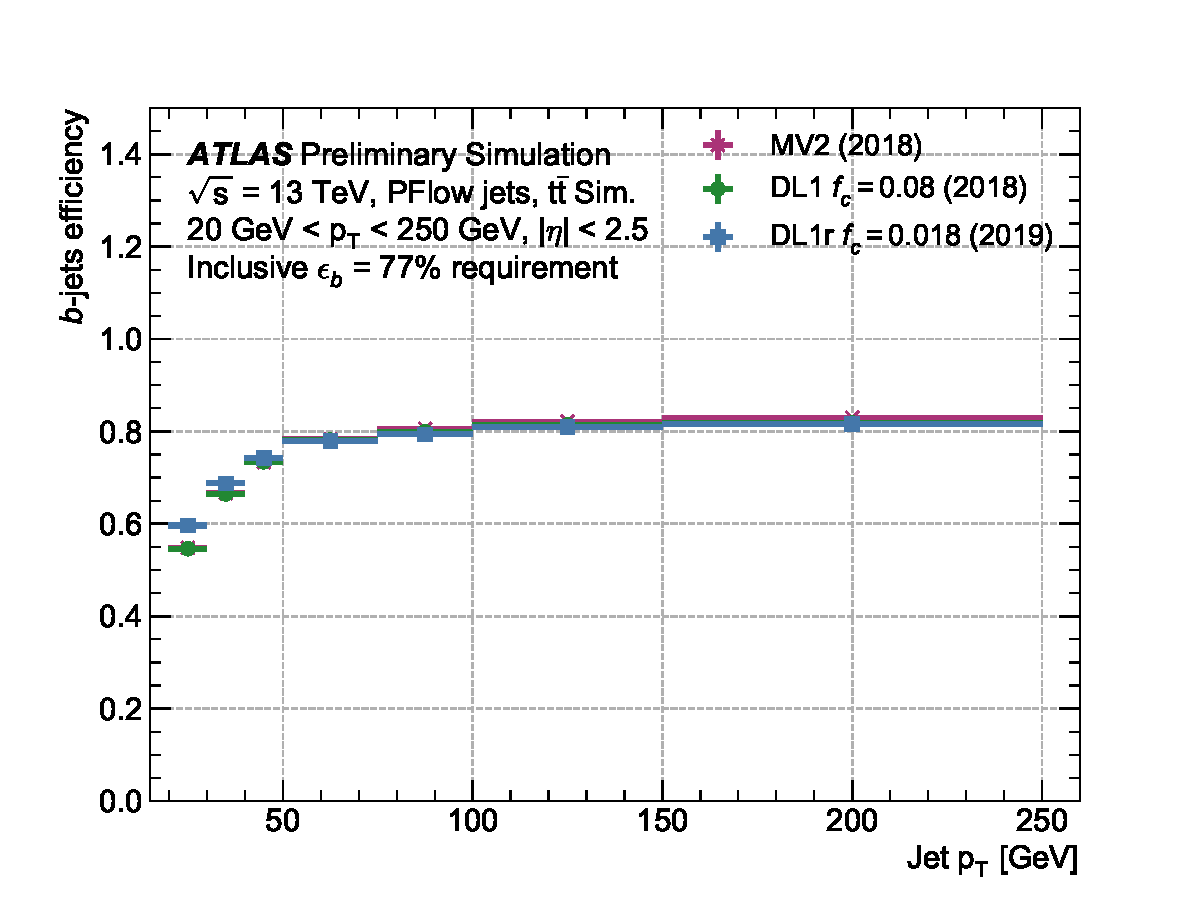
\includegraphics[width=.6\textwidth]{{figures/ftag/ATL-PHYS-PUB-2018-025/fig_02a.pdf}} 
% Note fig (b) shows the reconstruction level picture
\caption{\cite{ATL-PHYS-PUB-2018-025}}
\label{fig:jf-fig-02a}
\end{figure}

The tracks fed in as input to the JF algorithm have a loose selection criteria of $|d_0| < 3.5$~mm and $|z_0 \sin \theta| < 1.5$~mm, and $p_\text{T}^{trk} > 500~$MeV. 
The Kalman Filter formalism is extended to fit a number of secondary vertices, with the extended state vector (of the Hidden Markov Model) given by \Eq{\ref{eq:jf-state}}.
The key assumption of this algorithm is that all of the displaced vertices lie on the \emph{same} flight axis, characterized by the $(\phi,\theta)$ direction.
Then the cascade of $N$ displaced vertices are identified by the distance along this flight path from the PV (denoted by the $d_1, d_2, \ldots d_N$ distances).

\begin{equation}
\vec{d} = \left( x_{PV}, y_{PV}, z_{PV}, \phi, \theta, d_1, d_2, \ldots, d_N \right)
\label{eq:jf-state}
\end{equation}

The jet axis is used to initialize $(\phi,\theta)$, and the N displaced vertices are considered for the tracks intersecting this flight axis. % p117 of G's thesis

The set of input variables that characterize the result of the multi-vertex fit are listed in \Tab{\ref{tab:jf-inpus}}. There are two types of input variables. 
The first 8 variables listed in  \Tab{\ref{tab:jf-inpus}} characterize the properties of the tracks in the full cascade fit. 
The mass of the tracks also includes a constraint from conservation of momentum to account for the neutral tracks and improve the mass resolution (see \Sect{\ref{sec:jf-mass-constraint}} for further details). A subset of these variables is shown in \Fig{\ref{fig:jf-inputs}}.

\def\figpath{figures/ftag/ANA-FTAG-2019-07-PAPER/jetfitter}
\begin{figure}[htbp]
\centering
\subfloat[]{ 
    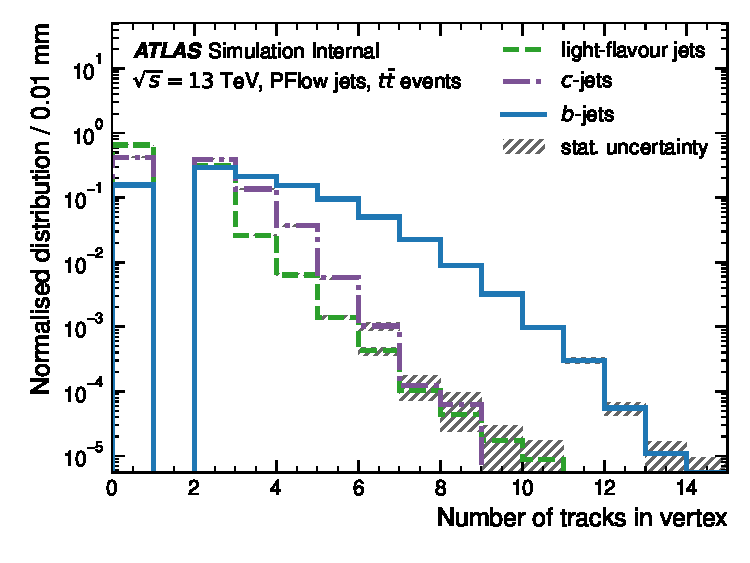
\includegraphics[width=0.32\linewidth]{\figpath/JetFitter_nTracksAtVtx_ttbar.pdf}
} 
\subfloat[]{ 
    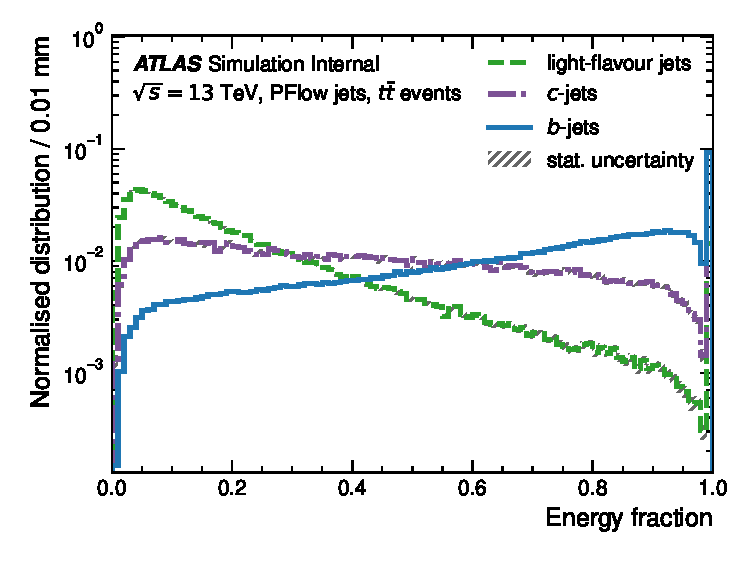
\includegraphics[width=0.32\linewidth]{\figpath/JetFitter_energyFraction_ttbar.pdf}
} 
     \subfloat[]{ 
    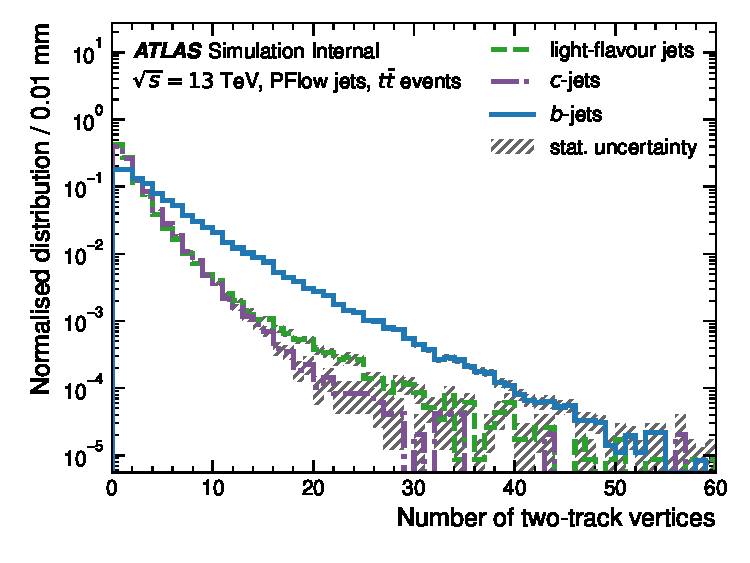
\includegraphics[width=0.32\linewidth]{\figpath/JetFitter_N2Tpair_ttbar.pdf}
} \\ 
\subfloat[]{ 
    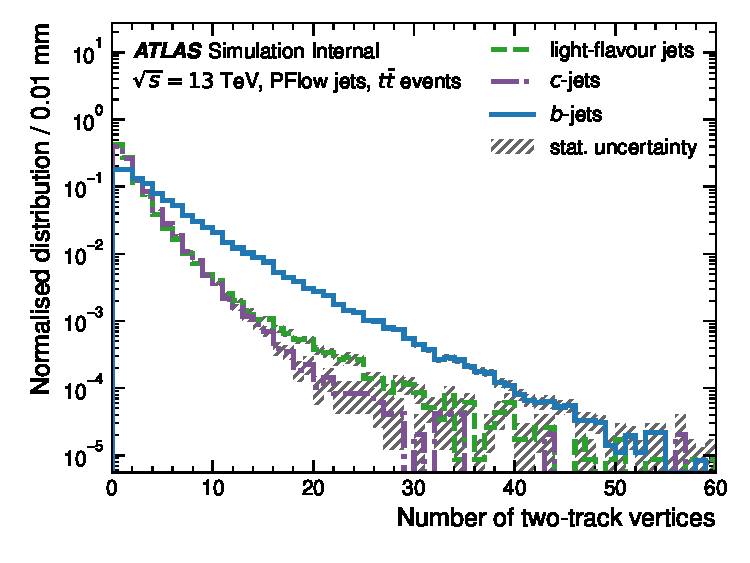
\includegraphics[width=0.32\linewidth]{\figpath/JetFitter_N2Tpair_ttbar.pdf}
} 
\subfloat[]{ 
    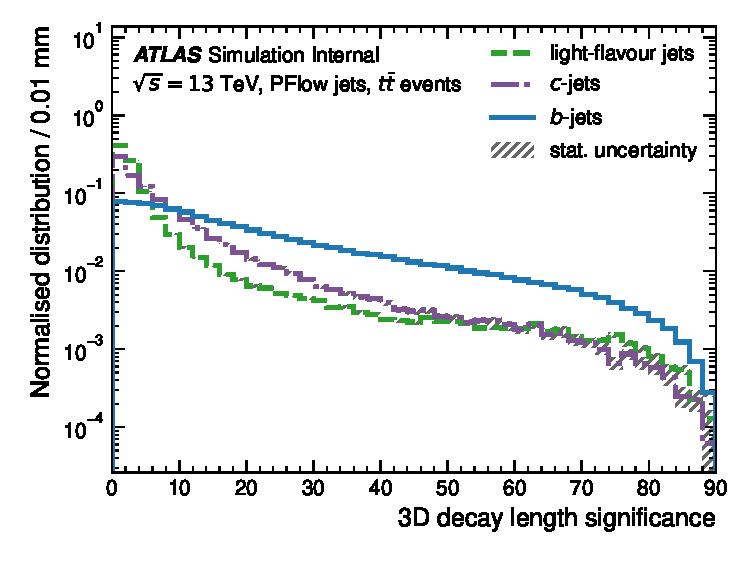
\includegraphics[width=0.32\linewidth]{\figpath/JetFitter_significance3d_ttbar.pdf}
} 
\subfloat[]{ 
    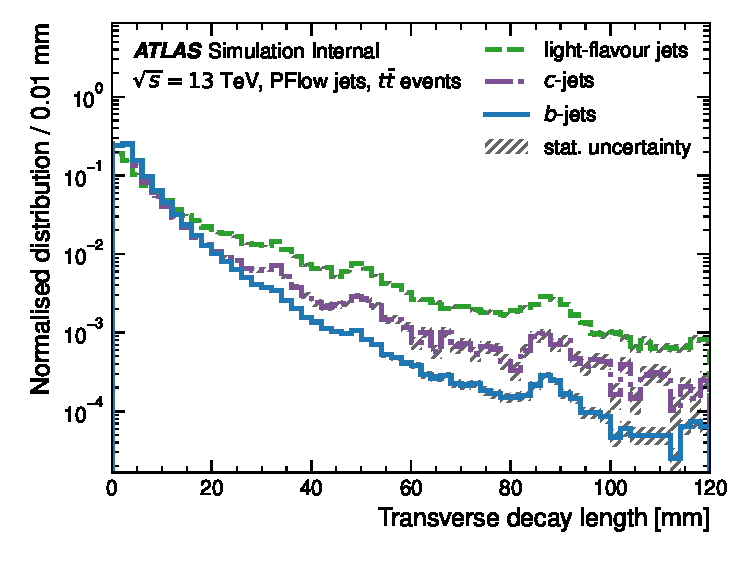
\includegraphics[width=0.32\linewidth]{\figpath/JetFitterSecondaryVertex_displacement2d_ttbar.pdf}
} 
\caption{An illustration of some of the JF inputs \cite{ANA-FTAG-2019-07}.}
\label{fig:jf-inputs}
\end{figure}


The second block of variables were included to optimize the sensitivity to \Pqc-tagging. For \Pqb-jets, we only expect one displaced vertex, so these variables are only calculated when JF finds \emph{exacly one} displaced vertex. These variables quantify the (2d and 3d) distance of the SV, its invariant mass, the energy of the trakcs and track muliplicity of the displaced vertex. 
Additionally, since the \Pqc-hadron has a lower decay multiplicity than the \Pqb-hadron decay, this means each of the \Pqc-hadron tracks carry a larger proportion of the energy and have a wider opening angle \cite{ATL-PHYS-PUB-2017-013}. 
The min, max, and avg $\eta$ of the tracks in the jet and the tracks in the displaced vertex and the tracks in the jet give us a handle on this discrimination variable.

\begin{table}[h!]
\centering
\begin{tabular}{p{3cm} | p{11cm}  } 
\textbf{Input} & \textbf{Description}  \\
\hline
\hline
	$m_{JF}$ & Invariant mass of the tracks attached to displaced vertices \\
	$f_E$ & Fraction of the energy in the displaced vertices compared to the jet's energy \\
	$\Delta R(\vec{p}_{jet}, \vec{p}_{vtx})$ & \\
	$S_{xyz}$ & Average significance of all of the displaced vertices \\
	$N_{trk}$ & Number of tracks associated to the fitted displaced vertices along the cascade decay chain \\
	$N_{2-\text{trk-vtx}}$ & Number of 2 track vertices (before the decay chain fit) \\
	$N_{1-\text{trk-vtx}}$ & Number of the single track vertices (after the decay chain fit) \\
	$N_{\geq 2-\text{trk-vtx}}$ & Number of the multi-prong displaced vertices (after the decay chain fit) \\
	\hline
	$L_{xyz}$(SV) & 3d distance from the first displaced vertex  \\
	$L_{xy}$(SV) &  transverse distance from the first displaced vertex \\
	$m_{trk}$(SV) & Mass of the tracks associated to the first displaced vertex \\
	$E_{trk}$(SV) & Energy of the tracks in the first displaced vertex \\
	$f_E$(SV) & Energy fraction of the tracks in the first displaced vertex compared to the energy of the jet \\ 
	$N_{\text{trk}}$(SV) & Number of tracks attached to the first displaced vertex \\
	$\eta_{\text{trk}}^{\text{max, min, avg}}$(SV) & The maximum, minimum, and average pseudorapidity of the tracks in the displaced vertex \\
	$\eta_{\text{trk}}^{\text{max, min, avg}}$ & The maximum, minimum, and average pseudorapidity of the tracks in the jet\\	
	% Are these abs etas or w/r.t. the jet axis?
\end{tabular}
\caption{Features from the JF reconstruction that are fed as input to the DL1r tagger. The first block of variables quantifies the global properties of the displaced vertices and decay topology. The second set of variables just looks at the properties of the first displaced vertex which capture the differences between \Pqb-jets and \Pqc-jets.}
\label{tab:jf-inputs}
\end{table}


